\documentclass[12pt,a4paper,oneside]{report}

\usepackage{iftex}
\ifPDFTeX
  \usepackage[T1]{fontenc}
  \usepackage{newtxtext,newtxmath}
\else
  \usepackage{fontspec}
  \IfFontExistsTF{Times New Roman}
    {\setmainfont{Times New Roman}}
    {\setmainfont{TeX Gyre Termes}}
\fi

\usepackage[left=1.5in,right=1in,top=1in,bottom=1in]{geometry}
\usepackage{setspace}
\usepackage{ragged2e}
\usepackage{graphicx}
\usepackage{booktabs}
\usepackage{longtable}
\usepackage{array}
\usepackage{tabularx}
\usepackage{amsmath}
\usepackage{chngcntr}
\usepackage{caption}
\usepackage{enumitem}
\usepackage{fancyhdr}
\usepackage{titlesec}
\usepackage{tikz}
\usetikzlibrary{positioning,arrows.meta,shapes.geometric}
\usepackage[numbers,sort&compress]{natbib}
\usepackage[hidelinks]{hyperref}

\setstretch{1.5}
\justifying
\setlength{\parindent}{0.5in}
\setlength{\parskip}{0pt}
\setlist{itemsep=0.2em,topsep=0.3em}
\counterwithin{figure}{chapter}
\counterwithin{table}{chapter}
\numberwithin{equation}{chapter}
\captionsetup{font=small,labelfont=bf}
\renewcommand{\arraystretch}{1.2}
\titleformat{\chapter}[display]
  {\normalfont\bfseries\centering\fontsize{16}{20}\selectfont}
  {\chaptername\ \thechapter}{0.5em}{}
\titleformat{\section}
  {\normalfont\bfseries\fontsize{14}{17}\selectfont}
  {\thesection}{0.75em}{}
\titleformat{\subsection}
  {\normalfont\bfseries\fontsize{14}{17}\selectfont}
  {\thesubsection}{0.75em}{}

\pagestyle{fancy}
\fancyhf{}
\fancyhead[L]{AI Student Learning Assistant}
\fancyhead[R]{\nouppercase{\leftmark}}
\fancyfoot[C]{\thepage}
\setlength{\headheight}{15pt}
\renewcommand{\chaptermark}[1]{\markboth{#1}{}}

\newcommand{\placeholder}[1]{\textit{[ #1 ]}}
\newcolumntype{Y}{>{\raggedright\arraybackslash}X}

\begin{document}
\begin{titlepage}
  \centering
  \vspace*{1.3in}
  {\bfseries\fontsize{20}{24}\selectfont AI STUDENT LEARNING ASSISTANT\par}
  \vspace{0.35in}
  {\bfseries\fontsize{16}{20}\selectfont Project Report\par}
  \vspace{0.7in}
  {\large Submitted in partial fulfilment of the requirements for\par}
  \vspace{0.15in}
  {\large\bfseries \placeholder{Degree / Programme Name}\par}
  \vspace{0.75in}
  \begin{tabular}{rl}
    \textbf{Submitted by:} & \placeholder{Student name(s) and registration number(s)}\\[0.35em]
    \textbf{Department:} & \placeholder{Department name}\\[0.35em]
    \textbf{Institution:} & \placeholder{University / institution name}\\[0.35em]
    \textbf{Project guide:} & \placeholder{Guide name and designation}\\[0.35em]
    \textbf{Academic year:} & \placeholder{Academic year}
  \end{tabular}
  \vfill
  {\large \placeholder{City, State, Country}\par}
  \vspace{0.15in}
  {\large \today\par}
\end{titlepage}

\pagenumbering{roman}
\chapter*{Certificate}
\addcontentsline{toc}{chapter}{Certificate}
This is to certify that the project report entitled \textit{AI Student Learning Assistant} describes the software implementation examined in this report and is submitted by \placeholder{Student name(s) and registration number(s)} in partial fulfilment of the requirements for \placeholder{Degree / Programme Name}. The institutional certification, approval, signatures, and dates must be completed by the relevant academic authorities.

\vspace{1.2in}
\noindent
\begin{tabularx}{\textwidth}{YY}
\placeholder{Project guide signature and date} & \placeholder{Head of department signature and date}\\[1.1in]
\placeholder{External examiner signature and date} & \placeholder{Institution seal, if required}
\end{tabularx}

\chapter*{Declaration}
\addcontentsline{toc}{chapter}{Declaration}
I / We declare that this report is prepared for academic submission and that all statements about the software are grounded in the project files cited or described herein. Any institutional declaration concerning originality, prior submission, authorship, or permitted use of external material must be reviewed and completed by the submitting student(s) in accordance with university policy.

\vspace{0.8in}
\noindent
\placeholder{Student name(s)} \hfill \placeholder{Signature(s)}\\[0.5em]
\placeholder{Place and date}

\chapter*{Acknowledgements}
\addcontentsline{toc}{chapter}{Acknowledgements}
\placeholder{Add acknowledgements for the project guide, department, institution, collaborators, and other contributors. No personal acknowledgements were present in the inspected project files.}

\chapter*{Abstract}
\addcontentsline{toc}{chapter}{Abstract}
The AI Student Learning Assistant is a Python application intended to support study activities using user-uploaded PDF material. The inspected implementation combines a Streamlit interface, a PDF text-extraction path based on \texttt{pypdf}, a word-based overlapping text splitter, normalized sentence embeddings from the configured Sentence Transformers model, a FAISS flat L2 index, a lexical-and-dense retrieval stage, and a LangGraph state graph that dispatches work to task-specific prompt and agent functions. The interface offers topic explanation, quiz, flashcard, summary, study-planner, and chat selections. Generated responses are sent through a Groq chat-model wrapper when credentials are available, and the interface displays retrieval-derived source/page information, a heuristic confidence value, and elapsed query time.

The report documents the source-backed architecture, configuration, algorithms, implementation, and two test cases present in the repository. It distinguishes implementation evidence from performance or learning outcomes: the project contains no benchmark dataset, measured quality results, user study, deployment evidence, or generated application screenshots. The existing tests cover a basic splitter output and response-text sanitization only. Accordingly, no accuracy, educational effectiveness, latency target, or production-readiness claim is made. Several gaps relevant to operation and future evaluation are identified, including replacement of the current index on each PDF indexing call, the absence of an OCR path, and the limited scope of the existing tests.

\noindent\textbf{Keywords:} Retrieval-augmented generation; educational assistant; PDF processing; dense embeddings; FAISS; hybrid retrieval; LangGraph; Streamlit.

\tableofcontents
\listoffigures
\listoftables
\clearpage
\pagenumbering{arabic}

\chapter{Introduction}
\label{ch:introduction}

\section{Context}
Students commonly study from course notes, textbooks, and lecture documents whose content is specific to a course or instructor. A general-purpose language model may answer outside that local material, while manual search through long documents can interrupt study. Retrieval-augmented generation (RAG) is a software pattern in which relevant passages are retrieved from a knowledge collection and supplied to a language model when responding. The foundational RAG formulation combines parametric generation with non-parametric retrieved memory \citep{lewis2020rag}.

The project applies this pattern to PDF-based study material. A student uploads documents, selects a learning task, and submits a topic or question. The implementation extracts text, divides it into chunks, embeds those chunks for semantic search, ranks candidates using dense and lexical signals, and passes the selected context to one task-oriented response function.

\section{Project overview}
The repository implements a local Streamlit application in Python. Its runtime is assembled from a user interface, a RAG pipeline, a compiled LangGraph state graph, task-specific agents and prompt builders, a Groq model adapter, and shared utility functions. LangGraph is used as explicit state-and-control-flow orchestration rather than as evidence of multiple autonomous model loops \citep{langgraphdocs}.

The application's visible task choices in \texttt{app.py} are Explain Topic, Generate Quiz, Generate Flashcards, Generate Summary, Study Planner, and Chat. Six agent functions are defined in the source, including a doubt solver. The distinction between implemented agent code and choices that can be selected in the interface is discussed in Chapter~\ref{ch:implementation}.

\section{Motivation and significance}
The project addresses a practical software problem: making a user's own study documents searchable through natural-language requests and adapting the requested response format to study activities. Its educational value is a design intention, not a measured outcome. No user evaluation, comparison with a baseline, or learning assessment is included in the repository.

\section{Scope}
This report covers source files, configuration, dependencies, tests, and the README found in the inspected repository. The active application path handles text-based PDF extraction, local embedding and FAISS persistence, retrieval, model invocation through Groq, and Streamlit presentation. It does not claim OCR support, multi-user access control, a hosted deployment, or a tested end-to-end educational intervention.

\section{Report organization}
Chapter~\ref{ch:background} introduces the technologies and concepts evidenced by the implementation. Chapters~\ref{ch:problem}--\ref{ch:methodology} define the problem, requirements, architecture, and algorithmic method. Chapters~\ref{ch:implementation}--\ref{ch:testing} document the application and available verification. Chapters~\ref{ch:results}--\ref{ch:limitations} discuss evidence, security and ethics, and remaining gaps. Chapter~\ref{ch:conclusion} closes the report; appendices provide setup, configuration, a results-record template, and a source map.

\chapter{Background and Related Concepts}
\label{ch:background}

\section{Retrieval-augmented generation}
RAG combines retrieval of external context with language-model generation. In this application, the external collection is composed of chunks extracted from uploaded PDFs, and the retrieved text is inserted into a task-specific prompt. The source code instructs the model to treat that material as reference and to avoid answering when it is insufficient. This is a prompt-level design; it does not prove that every generated statement is grounded or that unsupported content is impossible.

\section{PDF text extraction}
The active extraction helper uses \texttt{pypdf.PdfReader}, iterates pages starting at page 1, calls \texttt{extract\_text()}, and omits pages whose extracted text is empty. The \texttt{pypdf} documentation describes extraction as parsing page content streams and notes that image-only pages may not yield usable text \citep{pypdfdocs}. The repository does not implement an OCR stage.

\section{Embedding-based retrieval}
The configured model name is \texttt{sentence-transformers/all-MiniLM-L6-v2}. Its model card describes a 384-dimensional dense vector representation used for tasks including semantic search \citep{minilmcard}. The code requests normalized embeddings and converts them to NumPy \texttt{float32}. These embeddings provide a semantic representation for indexed chunks and queries.

\section{FAISS vector search}
FAISS provides data structures and operations for vector similarity search \citep{faissdocs}. The project creates \texttt{faiss.IndexFlatL2} with a configured dimension of 384, adds vectors, and requests nearest neighbors using the L2 index. This is an exact flat index implementation in the code; no approximate index or external vector database is configured.

\section{Hybrid retrieval}
The active retriever combines a dense-distance-derived score with a lightweight keyword-overlap score. This hybrid design can use semantic similarity and exact term matches as complementary signals. In this implementation, it is a custom ranking procedure over an in-process FAISS index and Python metadata, not a separately deployed search service.

\section{Workflow orchestration and user interface}
LangGraph represents workflows using shared state, nodes, and edges; its documentation presents the framework as a low-level orchestration runtime \citep{langgraphdocs}. Here, a router node selects one of six agent nodes, each of which calls its own prompt builder and writes a response into the shared state. Streamlit reruns scripts in response to interactions and provides resource caching and session state; the project uses \texttt{st.cache\_resource} for its graph and RAG pipeline and \texttt{st.session\_state} for conversation history \citep{streamlitcache}.

\section{Model-provider integration}
The model wrapper lazily constructs LangChain's \texttt{ChatGroq} integration using the configured model name and API key, then invokes it with a prompt string. The provider integration is documented by LangChain \citep{chatgroqdocs}. Actual successful model access depends on a valid credential, provider availability, and model availability; the repository contains no recorded provider response or integration test.

\chapter{Problem Definition and Objectives}
\label{ch:problem}

\section{Problem statement}
The project targets the effort required to locate relevant content in a student's own PDF study material and restate that content in formats useful for revision. The software problem is to connect document ingestion, query-time retrieval, task selection, model prompting, and display while retaining basic source and page metadata.

\section{Objectives}
\begin{enumerate}
  \item Accept PDF study files through a browser-based interface.
  \item Extract page text and preserve source and page identifiers for chunks.
  \item Build an embedding index and return relevant context for a query.
  \item Combine semantic and lexical evidence in a configurable ranking stage.
  \item Route the selected task to a matching prompt and agent function.
  \item Present an answer together with retrieval-source details and simple runtime indicators.
\end{enumerate}
These objectives describe intended software behavior. The available tests do not establish that all objectives pass end-to-end.

\section{Inputs and outputs}
Inputs consist of PDF files and a text request selected from a UI task mode. The primary output is Markdown-like model text. The application also exposes a confidence heuristic, elapsed query time, source names, page values, relevance values, and a citation preview based on retrieved metadata. It does not produce a formally formatted bibliographic citation for the source PDFs.

\section{Assumptions and boundaries}
The ingestion path assumes a PDF from which \texttt{pypdf} can extract text. It assumes the embedding model can be loaded in the local environment and that vector dimensions match the configured index dimension. Live generation assumes a usable Groq API key. There is no project evidence that scanned documents, malformed files, concurrent users, or large-scale collections have been evaluated.

\section{Success criteria and evidence}
The source establishes the intended flow and two small unit-level assertions. It does not define measurable acceptance thresholds for retrieval relevance, answer correctness, response latency, or learning benefit. Such criteria should be defined before a formal evaluation; a data-record template is provided in Appendix~\ref{app:evaluation}.

\chapter{Requirements Analysis}
\label{ch:requirements}

\section{Functional requirements}
\begin{longtable}{p{0.12\textwidth}p{0.48\textwidth}p{0.30\textwidth}}
\caption{Functional requirements and source evidence}\label{tab:functional-requirements}\\
\toprule
\textbf{ID} & \textbf{Requirement} & \textbf{Evidence / qualification}\\
\midrule
\endfirsthead
\toprule
\textbf{ID} & \textbf{Requirement} & \textbf{Evidence / qualification}\\
\midrule
\endhead
FR-01 & Upload one or more PDF files in the browser interface. & \texttt{st.file\_uploader}; the indexing loop processes selected files serially.\\
FR-02 & Extract text and page metadata from PDF pages. & \texttt{extract\_pdf\_text}; empty pages are omitted.\\
FR-03 & Divide text into overlapping chunks and embed them. & Active splitter uses word counts; default size 1200 and overlap 200.\\
FR-04 & Retrieve relevant context for a question. & Hybrid retriever uses FAISS distance and keyword overlap.\\
FR-05 & Generate task-oriented responses. & Six agent functions and six prompt templates exist.\\
FR-06 & Show response and source-related metadata. & UI displays confidence, duration, sources, pages, relevance, and citation preview.\\
FR-07 & Retain conversation history during interaction. & History is stored in Streamlit session state; no external history database is configured.\\
\bottomrule
\end{longtable}

\section{Non-functional considerations}
\begin{longtable}{p{0.20\textwidth}p{0.43\textwidth}p{0.27\textwidth}}
\caption{Non-functional considerations evidenced or left open}\label{tab:nfr}\\
\toprule
\textbf{Concern} & \textbf{Observed implementation} & \textbf{Evidence gap}\\
\midrule
\endfirsthead
\toprule
\textbf{Concern} & \textbf{Observed implementation} & \textbf{Evidence gap}\\
\midrule
\endhead
Configurability & Model, chunk parameters, top-$k$, and hybrid weight can be set with environment variables. & No validation ranges are specified for every parameter.\\
Persistence & FAISS index and metadata are written beneath \texttt{vector\_store}. & No backup, migration, or multi-user isolation scheme is included.\\
Observability & Application log file and UI timing/confidence indicators are present. & No structured trace, monitoring service, or calibrated confidence evaluation.\\
Security & API key is loaded from environment; \texttt{.env} is ignored by Git. & No authentication or security test suite is present.\\
Usability & Streamlit provides upload, task selection, query input, and answer display. & No user study or accessibility evaluation is included.\\
Performance & Resource caching avoids recreating the graph and pipeline on every rerun. & No throughput, memory, or latency benchmark is supplied.\\
\bottomrule
\end{longtable}

\section{Software and dependency requirements}
The dependency declarations in \texttt{requirements.txt} are minimum version constraints, not a locked environment. The repository does not specify a Python version. Table~\ref{tab:dependencies} summarizes the packages and source-backed roles.

\begin{table}[htbp]
\centering
\caption{Declared software dependencies}
\label{tab:dependencies}
\begin{tabularx}{\textwidth}{p{0.27\textwidth}p{0.18\textwidth}Y}
\toprule
\textbf{Package} & \textbf{Minimum} & \textbf{Role in project}\\
\midrule
Streamlit & 1.37.0 & Browser-based interface and session state.\\
LangChain & 0.3.0 & Model integration ecosystem dependency.\\
LangGraph & 0.2.0 & Stateful graph orchestration.\\
LangChain-Groq & 0.2.0 & Groq chat-model adapter.\\
Sentence Transformers & 3.0.0 & Dense text embeddings.\\
faiss-cpu & 1.8.0 & Local vector index.\\
pypdf & 4.0.0 & PDF text extraction.\\
python-dotenv & 1.0.0 & Loading environment values from \texttt{.env}.\\
NumPy & 1.26.0 & Embedding arrays and numeric conversion.\\
\bottomrule
\end{tabularx}
\end{table}

\section{Hardware and deployment requirements}
The repository does not specify minimum CPU, RAM, disk, GPU, or network requirements, and it does not contain deployment manifests or a hosted-service configuration. Embedding model loading and external Groq generation have runtime and connectivity implications, but their minimum resource needs are not measured here. These values should be established on the target deployment environment rather than inferred from the source.

\chapter{System Design}
\label{ch:design}

\section{Architectural overview}
Figure~\ref{fig:architecture} shows the two major flows. PDF ingestion creates a local vector index and metadata collection; query handling retrieves context, routes the task, calls the selected agent, and displays the response. The diagram reflects the active imports and calls in \texttt{app.py}, \texttt{src/rag/rag\_pipeline.py}, and \texttt{src/graph/graph\_builder.py}.

\begin{figure}[htbp]
\centering
\resizebox{0.98\textwidth}{!}{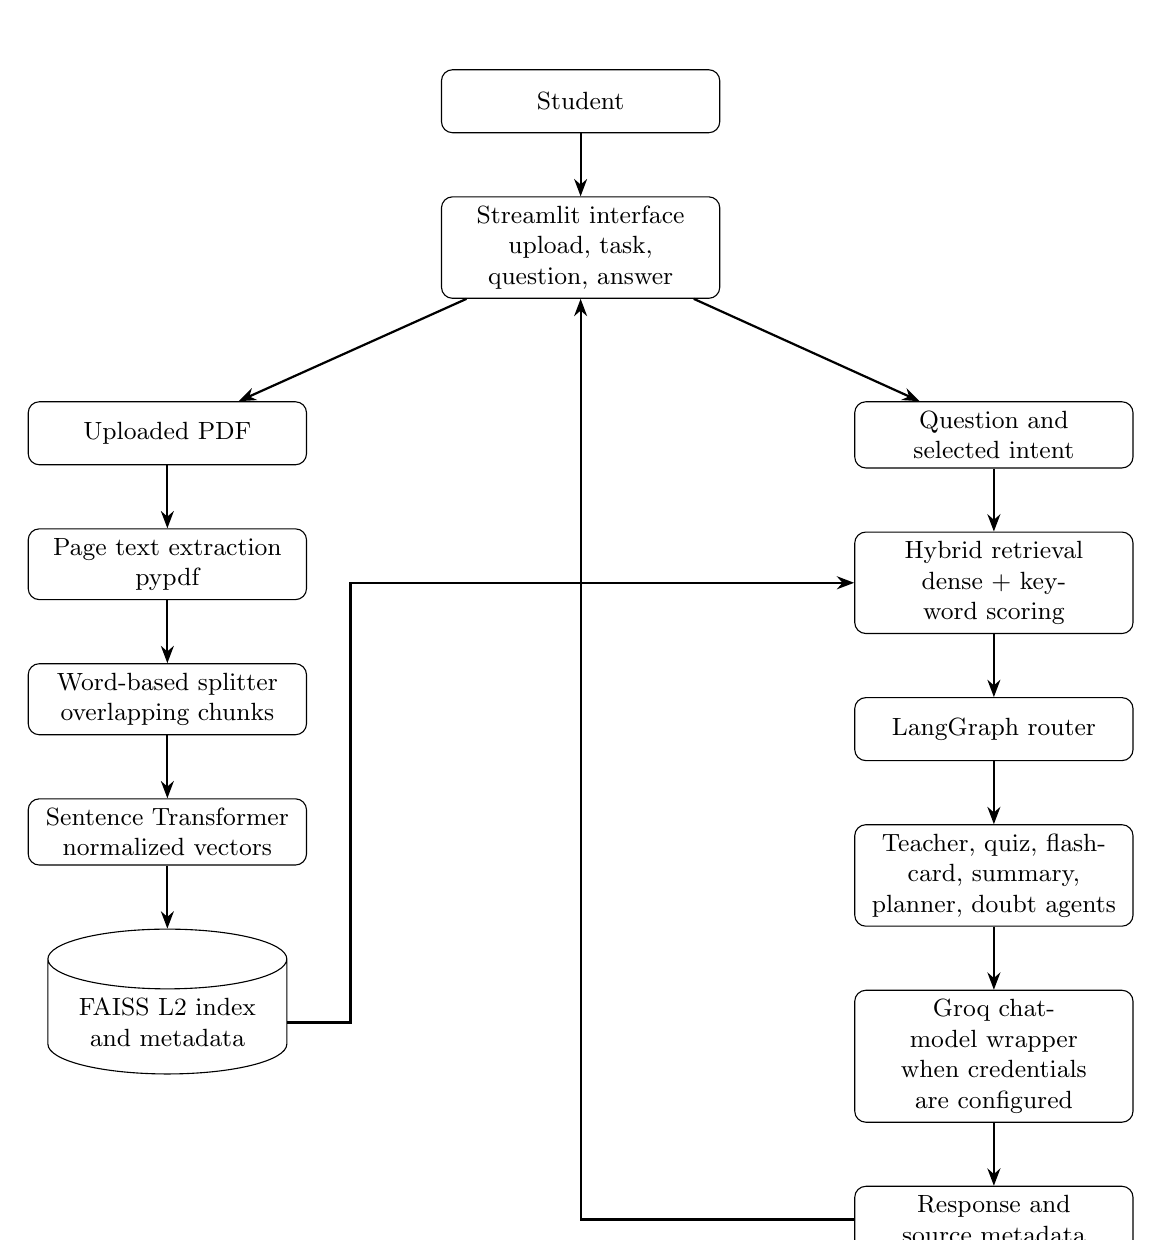
\begin{tikzpicture}[
  node distance=8mm and 11mm,
  block/.style={draw,rounded corners,align=center,text width=3.3cm,minimum height=0.8cm,font=\small},
  store/.style={draw,cylinder,shape border rotate=90,aspect=0.25,align=center,text width=2.8cm,minimum height=1.0cm,font=\small},
  flow/.style={-{Stealth[length=2.2mm]},thick},
  node distance=8mm
]
\node[block] (student) {Student};
\node[block,below=of student] (ui) {Streamlit interface\\upload, task, question, answer};
\node[block,below left=13mm and 17mm of ui] (pdf) {Uploaded PDF};
\node[block,below=of pdf] (extract) {Page text extraction\\pypdf};
\node[block,below=of extract] (split) {Word-based splitter\\overlapping chunks};
\node[block,below=of split] (embed) {Sentence Transformer\\normalized vectors};
\node[store,below=of embed] (index) {FAISS L2 index\\and metadata};
\node[block,below right=13mm and 17mm of ui] (query) {Question and selected intent};
\node[block,below=of query] (retrieve) {Hybrid retrieval\\dense + keyword scoring};
\node[block,below=of retrieve] (router) {LangGraph router};
\node[block,below=of router] (agents) {Teacher, quiz, flashcard, summary, planner, doubt agents};
\node[block,below=of agents] (llm) {Groq chat-model wrapper\\when credentials are configured};
\node[block,below=of llm] (response) {Response and source metadata};

\draw[flow] (student) -- (ui);
\draw[flow] (ui) -- (pdf);
\draw[flow] (pdf) -- (extract);
\draw[flow] (extract) -- (split);
\draw[flow] (split) -- (embed);
\draw[flow] (embed) -- (index);
\draw[flow] (ui) -- (query);
\draw[flow] (query) -- (retrieve);
\draw[flow] (index.east) -- ++(8mm,0) |- (retrieve.west);
\draw[flow] (retrieve) -- (router);
\draw[flow] (router) -- (agents);
\draw[flow] (agents) -- (llm);
\draw[flow] (llm) -- (response);
\draw[flow] (response.west) -| (ui.south);
\end{tikzpicture}
}
\caption{Source-backed system architecture of the application}
\label{fig:architecture}
\end{figure}

\section{Component responsibilities}
\begin{table}[htbp]
\centering
\caption{Main runtime components}
\label{tab:components}
\begin{tabularx}{\textwidth}{p{0.27\textwidth}Y}
\toprule
\textbf{Component} & \textbf{Responsibility}\\
\midrule
\texttt{app.py} & Streamlit controls, uploaded-file persistence, task selection, query orchestration, and answer display.\\
\texttt{config.py} & Environment-backed defaults, filesystem paths, and directory creation.\\
\texttt{src/rag} active path & PDF text loading, splitting, embedding, FAISS persistence, hybrid retrieval, and RAG coordination.\\
\texttt{src/graph} & Shared state schema, intent router, agent nodes, and graph compilation.\\
\texttt{src/agents} and \texttt{src/prompts} & Task-specific prompt construction, model invocation, response sanitization, and confidence assignment.\\
\texttt{src/models/llm.py} & Lazy Groq chat-model adapter and user-readable fallback strings.\\
\texttt{src/utils} & Source formatting, prompt instruction, response sanitization, confidence heuristic, PDF extraction, and logging.\\
\bottomrule
\end{tabularx}
\end{table}

\section{Data and control flow}
The compiled graph contains a router node and six terminal agent nodes. The router selects one node from the value returned by \texttt{route\_query}; each task agent consumes the retrieved documents, assembles their text as prompt context, invokes a model wrapper when context is non-empty, and updates the shared state. Figure~\ref{fig:query-workflow} summarizes query-time execution.

\begin{figure}[htbp]
\centering
\resizebox{0.98\textwidth}{!}{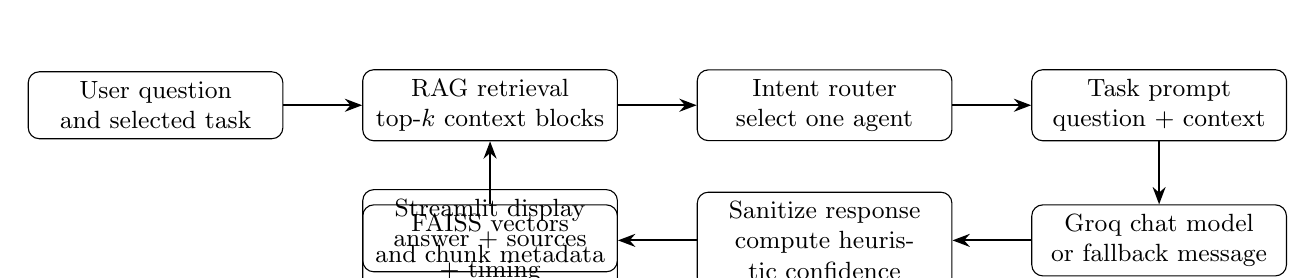
\begin{tikzpicture}[
  node distance=8mm and 10mm,
  block/.style={draw,rounded corners,align=center,text width=3.0cm,minimum height=0.85cm,font=\small},
  flow/.style={-{Stealth[length=2.2mm]},thick}
]
\node[block] (input) {User question\\and selected task};
\node[block,right=of input] (retrieve) {RAG retrieval\\top-$k$ context blocks};
\node[block,right=of retrieve] (route) {Intent router\\select one agent};
\node[block,right=of route] (prompt) {Task prompt\\question + context};
\node[block,below=of prompt] (model) {Groq chat model\\or fallback message};
\node[block,left=of model] (clean) {Sanitize response\\compute heuristic confidence};
\node[block,left=of clean] (display) {Streamlit display\\answer + sources + timing};
\node[block,below=of retrieve] (index) {FAISS vectors\\and chunk metadata};

\draw[flow] (input) -- (retrieve);
\draw[flow] (index) -- (retrieve);
\draw[flow] (retrieve) -- (route);
\draw[flow] (route) -- (prompt);
\draw[flow] (prompt) -- (model);
\draw[flow] (model) -- (clean);
\draw[flow] (clean) -- (display);
\end{tikzpicture}
}
\caption{Query-time workflow from user input to displayed answer}
\label{fig:query-workflow}
\end{figure}

\section{State model}
The \texttt{AgentState} TypedDict declares optional fields for the question, retrieved documents, intent, selected agent, response, sources, pages, chat history, confidence, routing label, response time, and retrieved chunk text. At runtime, \texttt{app.py} constructs this state before calling \texttt{graph.invoke}. The agent functions mutate and return the supplied dictionary; no external checkpoint store is configured.

\section{Persistence design}
The configured vector index path is \texttt{vector\_store/faiss.index}; metadata is stored in \texttt{vector\_store/metadata.pkl}. Uploaded PDFs are written to \texttt{data/uploads}. Both paths are ignored by Git, as are logs. The application's conversation history is held in Streamlit session state rather than a durable database.

\chapter{Methodology and Algorithms}
\label{ch:methodology}

\section{Document ingestion}
For an uploaded file, the interface saves the bytes under \texttt{data/uploads/<filename>}. \texttt{PDFLoader} delegates to \texttt{extract\_pdf\_text}, which extracts each page independently and retains non-empty text with its source path and one-based page number. The pipeline then splits page text, embeds all resulting chunks, adds vectors and metadata to the FAISS index, and saves index state.

\section{Word-based chunking}
The active \texttt{RecursiveTextSplitter} tokenizes using Python's whitespace-based \texttt{split()}, rather than a model tokenizer or a character count. With defaults \(C=1200\) words and overlap \(O=200\) words, chunk \(j\) covers a word interval \([s_j,e_j)\), where the next start is \(s_{j+1}=e_j-O\) until the page is exhausted. Each chunk preserves source, page, and a generated chunk identifier. The configuration is adjustable through \texttt{CHUNK\_SIZE} and \texttt{CHUNK\_OVERLAP}.

\section{Dense vector representation}
Each chunk and query is encoded by the configured Sentence Transformer. The code calls \texttt{encode(..., normalize\_embeddings=True, convert\_to\_numpy=True)} and converts output to \texttt{float32}. The configured embedding dimension and FAISS index dimension are both 384. The code does not perform dimension discovery from the loaded model; therefore a model override must remain dimension-compatible.

\section{Hybrid candidate scoring}
The retriever asks FAISS for up to \(\max(3k,10)\) dense candidates, where \(k\) is the requested result count. For a returned L2 distance \(D(c,q)\), it derives a dense score:
\begin{equation}
S_{\mathrm{dense}}(c,q)=\frac{1}{1+\max(D(c,q),10^{-9})}.
\label{eq:dense-score}
\end{equation}
The lexical score counts query-term occurrences in a chunk and divides by the number of unique query terms:
\begin{equation}
S_{\mathrm{lex}}(c,q)=
\frac{\sum_{t\in T_q} f(t,c)}{\max(1,\lvert T_q\rvert)},
\label{eq:lexical-score}
\end{equation}
where \(T_q\) is the set of lower-cased word-like query terms and \(f(t,c)\) is their count in the chunk. Because occurrence counts are summed, the lexical score is not necessarily bounded by one.

The agreement term is a capped weighted fraction of dense candidates sharing the same source and page:
\begin{equation}
A(c)=\min\left(1,\;0.6\frac{n_s}{N}+0.4\frac{n_p}{N}\right),
\label{eq:agreement}
\end{equation}
where \(N\) is the number of dense results, \(n_s\) counts same-source results, and \(n_p\) counts same-page results. The initial combined score is:
\begin{equation}
S_0(c,q)=\alpha S_{\mathrm{dense}}(c,q)
+(1-\alpha)S_{\mathrm{lex}}(c,q)+0.05A(c).
\label{eq:hybrid-score}
\end{equation}
The default \(\alpha\) is 0.75. The implementation adds a source bonus of 0.06 for candidates from the source of the highest-scored candidate and a page bonus of \(0.04/(1+\Delta p)\), where \(\Delta p\) is the page distance from that reference candidate. Remaining metadata chunks are also considered with a lexical-only score. These constants are implementation heuristics; the repository provides no calibration or empirical justification for them.

\section{Context grouping and selection}
Ranked chunks are deduplicated by chunk ID, grouped when they share a source and have a page gap of at most one, and concatenated into context blocks. Each merged block is truncated to 2500 characters. Its displayed relevance, semantic, lexical, and agreement values are averages over its constituent entries. The resulting blocks are sorted and limited to \(k\). The summary branch calls the same merge function; it does not implement a distinct summary-ranking algorithm.

\section{Confidence heuristic}
For each retrieved document, the implementation computes a weighted sum:
\begin{equation}
C_i=0.35S_{\mathrm{semantic},i}
+0.25S_{\mathrm{keyword},i}
+0.20S_{\mathrm{agreement},i}
+0.20S_{\mathrm{relevance},i}.
\label{eq:confidence-item}
\end{equation}
It averages the document values, clamps the result to \([0,1]\), and rounds to two decimal places. This number is presented as a confidence score, but is not calibrated against answer correctness and should be interpreted only as a retrieval-derived heuristic.

\section{Answer generation}
Each active agent builds a prompt containing a shared security instruction, task-specific output requirements, user question, and retrieved context. Empty context produces a fixed no-material response without calling the model. Otherwise, a Groq chat wrapper invokes the configured model. The answer is passed through a phrase-removal sanitizer before storage in graph state. The prompts request material-grounded answers, but the code does not apply a formal entailment check to the final answer.

\chapter{Implementation}
\label{ch:implementation}

\section{Application lifecycle}
The entry point is \texttt{app.py}. At import time it configures logging and ensures configured data, upload, vector-store, log, report, and test directories exist. The graph and RAG pipeline are each constructed by a function decorated with \texttt{st.cache\_resource}. Streamlit session state holds a list of question-answer pairs for the current interaction session.

\section{Document indexing behavior}
When the user selects \textit{Index PDFs}, the app loops over uploaded files and calls \texttt{RAGPipeline.index\_pdf}. That method clears the vector store before it loads and indexes the current file. Consequently, when multiple files are selected and indexed in one button operation, each subsequent file replaces the earlier file's vectors; after successful completion, only the last successfully indexed file remains in the index. This is the behavior of the current source, not a multi-document collection feature.

\section{Intent routing and agent set}
The interface converts its selected task label into a lower-case underscore-separated intent. The graph router checks for the substrings \texttt{quiz}, \texttt{flashcard}, \texttt{summary}, and \texttt{planner}; otherwise it selects the doubt solver only if the \emph{intent string} contains \texttt{doubt}, \texttt{why}, or \texttt{how}; all other cases select the teacher agent.

The UI choices include Chat and Explain Topic but not Doubt Solver. The natural-language question text is not consulted by \texttt{route\_query}; therefore, selecting Chat or Explain Topic routes to the teacher agent, and writing a question beginning with ``why'' does not by itself select the doubt solver. The doubt-solving agent is implemented but is not directly reachable through the current UI task list.

\section{Conversation history}
The question-answer history is retained in Streamlit session state and displayed below each response. The app also places that history in the graph state, but the task agents construct prompts from the current question and retrieved context only. Earlier turns are therefore shown in the interface but are not supplied as conversational context to the model.

\section{Task-oriented agents}
Six agent functions share a common structure: read retrieved document content, join it into context, call a task-specific prompt function, invoke \texttt{GroqChatModel}, sanitize the generated output, compute the same confidence heuristic, and set the selected-agent field. Prompt templates specify different output structures for explanation, doubt resolution, quiz, summary, planner, and flashcards. For example, the quiz prompt requests ten multiple-choice questions and the flashcard prompt requests ten cards. Those are model instructions, not guarantees that provider output will comply.

\section{Model adapter and failure behavior}
The wrapper defaults to \texttt{llama-3.3-70b-versatile} unless \texttt{GROQ\_MODEL} overrides it. The API key is read from the environment. If the optional integration cannot be imported or the key is absent, the wrapper returns a readable unavailability message; invocation exceptions are logged and converted to an error string. These fallback strings are displayed through the same response path and are not raised as application exceptions.

\section{Presentation and citations}
The interface renders the response as Markdown and displays a rounded elapsed time, source names, pages, and retrieved-block relevance. The citation preview formats source filename, page number, and optional section inferred from text. These are provenance hints derived from PDF metadata; they are not external citations or a bibliography.

\section{Logging and configuration}
Configuration is loaded from a repository-local \texttt{.env} file using \texttt{python-dotenv}, with process-environment values also available. Defaults include model name, embedding model, chunk size and overlap, top-$k$, and hybrid weight. The logger writes to \texttt{logs/application.log} and to the stream. The actual dependency declaration uses \texttt{pypdf}, although the repository README's technology table names PyMuPDF; the code and dependency file are the authoritative evidence for the active implementation.

\chapter{Testing and Verification}
\label{ch:testing}

\section{Tests present in the repository}
The repository contains one test module, \texttt{tests/test\_rag.py}, with two test functions:
\begin{enumerate}
  \item A splitter smoke test supplies one page of text and asserts that at least one chunk is returned.
  \item A response-sanitization test asserts that two prompt-like phrases are removed while a subsequent answer phrase remains.
\end{enumerate}
These tests do not exercise PDF parsing, embedding generation, vector persistence, hybrid ranking, LangGraph routing, Groq access, Streamlit interaction, multiple-file indexing, or end-to-end answer grounding.

\section{Validation performed for this report}
The available workspace has Python 3.13.2, but \texttt{pytest} is not installed; therefore the existing pytest suite could not be executed in this environment. No \texttt{pdflatex}, \texttt{latexmk}, \texttt{xelatex}, or \texttt{lualatex} executable was found. A compiled PDF could not be generated here. These are environment limitations, not evidence that the source tests or LaTeX report pass under a configured toolchain.

\section{Recommended verification plan}
Before release, the project should add unit tests for chunk boundaries and invalid parameters, page/source metadata, dense and lexical score behavior, deduplication and grouping, index save/load, and router selection. Integration tests should mock the embedding model and Groq client to cover graph invocation without network dependence. An application-level test should index multiple PDFs and assert the intended collection behavior. A separate evaluation should use a documented set of query-document relevance judgments and answer-grounding checks.

\section{LaTeX build verification}
The report is structured for Overleaf and XeLaTeX or LuaLaTeX. The main file includes package-level font fallback and uses ordinary BibTeX/natbib citations. Since a TeX engine is not available in the workspace, page layout, bibliography compilation, and figure rendering remain to be checked by compiling \texttt{main.tex} in Overleaf or another full LaTeX environment. Appendix~\ref{app:source-map} lists the report files for upload.

\chapter{Results and Discussion}
\label{ch:results}

\section{Implemented artifacts}
Source inspection confirms the existence of the PDF upload and indexing interface, configurable ingestion and retrieval components, a FAISS-backed vector store, a LangGraph router with six agent nodes, task-specific prompts, a Groq model wrapper, response display, and two small tests. The default configuration values and UI output fields are documented in Chapters~\ref{ch:requirements} and~\ref{ch:methodology}.

\section{Measured results}
No empirical result table, dataset, annotated relevance set, model-output corpus, user study, or benchmark script is included in the repository. Thus, there are no supported values for precision, recall, hit rate, answer faithfulness, quiz quality, learning gain, or performance targets. The UI computes elapsed response time and a retrieval-derived confidence heuristic at runtime, but neither is a recorded experimental result.

\begin{table}[htbp]
\centering
\caption{Evidence available and unavailable for evaluation}
\label{tab:evidence}
\begin{tabularx}{\textwidth}{p{0.38\textwidth}Y}
\toprule
\textbf{Measure / evidence} & \textbf{Status in inspected repository}\\
\midrule
Source-level architecture and configured defaults & Present in source files.\\
Splitter smoke test and sanitizer test & Present as two pytest test functions; execution unavailable because pytest is not installed in the workspace.\\
Retrieval relevance metrics & Not present.\\
Generation correctness or groundedness evaluation & Not present.\\
Latency or throughput benchmark & Not present; only a per-request UI timer is implemented.\\
Student usability or learning-outcome evaluation & Not present.\\
Compiled report PDF & Not generated; no TeX compiler found.\\
\bottomrule
\end{tabularx}
\end{table}

\section{Interpretation}
The implementation provides a coherent prototype path from document text to task-shaped responses, but the code alone cannot establish that retrieval is relevant, that model outputs obey their prompts, or that students learn more effectively. The index-clearing behavior also narrows the effective document collection when several PDFs are selected. Accordingly, this chapter reports implementation evidence rather than claiming experimental success.

\chapter{Security, Privacy, and Ethical Considerations}
\label{ch:security}

\section{Credential handling}
The Groq key is obtained through environment configuration, and \texttt{.env} is listed in \texttt{.gitignore}. This is a safer configuration pattern than embedding a key in source, but the repository does not show production secret management, key rotation, authorization, or deployment controls.

\section{Document handling and external processing}
Uploaded PDFs are saved under \texttt{data/uploads}; vector index and metadata are persisted locally. When live generation is configured, retrieved document text is included in a prompt sent through the Groq integration. The repository does not document provider data retention, user consent, a privacy notice, encryption at rest, deletion controls, or access separation. Deployers should disclose external processing and review provider terms before using sensitive course or student material.

\section{Prompt-injection and output controls}
Shared prompt instructions treat retrieved passages as untrusted reference material, instruct the model not to follow embedded directions, and limit responses to the uploaded material. A phrase-based output sanitizer removes configured strings. These are defense-in-depth intentions, not security proofs: the sanitizer is not a general detector, the tests cover only two phrases, and no adversarial evaluation is supplied. The project README's broader security claims should not be treated as verified guarantees.

\section{Persistence and file safety}
Metadata is deserialized using Python \texttt{pickle}. The application should only load metadata files from a trusted source; the repository does not implement integrity checks or a safe interchange format. The uploaded file name is used to form a destination path, and there is no explicit filename normalization in \texttt{save\_uploaded\_file}. Deployment review should consider path handling and storage permissions.

\section{Fairness, reliability, and academic use}
The model's responses may be incomplete, incorrect, or reflect biases in the underlying provider model. Retrieved source/page labels help users inspect supporting material but do not validate each statement. The displayed confidence is a heuristic, not a calibrated probability. Students should verify outputs against original course materials, especially for graded work, formulas, and safety-critical subject matter. No accessibility, bias, or educational-integrity evaluation is present.

\section{Security assessment boundary}
This chapter is a source-based discussion of design implications, not a penetration test, privacy audit, or formal security review. No claim is made that the application has been independently certified or is appropriate for deployment with confidential data.

\chapter{Limitations and Future Work}
\label{ch:limitations}

\section{Functional limitations}
\begin{itemize}
  \item \textbf{Index replacement:} \texttt{index\_pdf} clears the existing index for every file, so a sequence of uploads does not create a combined knowledge base.
  \item \textbf{Task routing mismatch:} the UI has no doubt-solving option, and the router sees the selected intent rather than the natural-language question.
  \item \textbf{Text-only PDF path:} there is no OCR stage for scanned pages; empty extraction results are skipped.
  \item \textbf{Persistence model:} the index is a local flat index with pickle metadata, without multi-user isolation, backup, or lifecycle management.
  \item \textbf{Prompt compliance:} desired formats and grounding rules are instructions to the LLM, not enforced output schemas.
\end{itemize}

\section{Retrieval and evaluation limitations}
The splitter uses words rather than model tokens and has no explicit validation of chunk-size/overlap consistency. The lexical term-count score can exceed one. The ranking weights and source/page bonuses have no documented tuning evidence. The confidence number is not empirically calibrated. The test suite is too small to characterize the full retrieval and generation pipeline, and no controlled evaluation results are included.

\section{Repository consistency}
The README names PyMuPDF, while the active implementation imports \texttt{pypdf} and \texttt{requirements.txt} declares \texttt{pypdf}. In addition, the repository contains alternate RAG modules (\texttt{chunker.py}, \texttt{pdf\_loader.py}, and \texttt{retriever.py}) that are not imported by the active pipeline and import \texttt{configure\_logging} from \texttt{config.py}; that function is not defined there. These files should be reconciled or removed in a future maintenance change. They are not represented as active components in the architecture figures.

\section{Prioritized future work}
\begin{enumerate}
  \item Preserve an existing index when adding a PDF, or expose an explicit replace/append collection choice; add a regression test for multiple files.
  \item Align the UI task options with router capabilities and test each route, including the intended behavior for Chat and doubt solving.
  \item Validate chunk parameters, normalize lexical scores, and compare ranking configurations against a labeled retrieval set.
  \item Add OCR as an optional documented path for scanned documents and test its page-level provenance.
  \item Add mocked end-to-end tests for retrieval, graph state, model fallbacks, and citations.
  \item Replace heuristic confidence presentation with a clearly labeled retrieval score or a separately calibrated confidence method.
  \item Define privacy, retention, access-control, and safe file-handling requirements before deployment.
  \item Reconcile the duplicate RAG modules and update README package descriptions to match the active dependency set.
\end{enumerate}

\chapter{Conclusion}
\label{ch:conclusion}

This report documented the AI Student Learning Assistant as it exists in the inspected repository. The application connects PDF text extraction and word-based chunking to normalized sentence embeddings, a local FAISS L2 index, custom hybrid retrieval, a LangGraph router, task-specific prompts, a Groq model wrapper, and a Streamlit user interface. The source also exposes source/page metadata, a retrieval-derived confidence heuristic, and a query timer.

The project demonstrates a useful integration of document search and task-oriented generation, but the available evidence is limited to implementation and two narrow tests. Multiple-file indexing currently replaces the prior index, the doubt-solver route is not directly exposed in the UI, scanned-PDF OCR is absent, and no systematic retrieval, generation, privacy, or learning evaluation is present. These limitations should be addressed before interpreting the system as a validated educational product or deploying it with sensitive documents.

The next engineering stage should first clarify and test the multi-PDF and intent-routing behavior, then add a controlled retrieval-and-grounding evaluation, operational privacy controls, and a reproducible build/test environment. Results from those activities can be added to the evaluation record in Appendix~\ref{app:evaluation}; until then, quantitative claims remain intentionally unreported.


\clearpage
\addcontentsline{toc}{chapter}{References}
\bibliographystyle{plainnat}
\bibliography{references}

\appendix
\chapter{Reproduction and Setup}
\label{app:setup}

\section{Environment preparation}
The repository README describes cloning the GitHub project, creating a Python virtual environment, installing the declared dependencies, creating a local \texttt{.env}, and launching Streamlit. The repository does not pin a Python release or dependency lockfile. Use the exact source checkout and record the Python and dependency versions used for any reproducible evaluation.

\section{Launch sequence}
\begin{enumerate}
  \item Create and activate a Python virtual environment appropriate for the operating system.
  \item Install the packages listed in the repository's \texttt{requirements.txt}.
  \item Copy \texttt{.env.example} to \texttt{.env} and configure a valid \texttt{GROQ\_API\_KEY} if live generation is required.
  \item Run \texttt{streamlit run app.py} from the project root.
  \item Upload a text-based PDF, select a task, submit a question, and inspect the answer and source/page display.
\end{enumerate}

\section{Reproducibility caveats}
Indexing uses local files and model downloads; live responses depend on a remote provider. The project does not define a deterministic model seed, pin exact package versions, include a sample PDF, or supply expected generated answers. Tests should mock external services when repeatability is required.

\chapter{Configuration Reference}
\label{app:configuration}

\begin{longtable}{p{0.27\textwidth}p{0.27\textwidth}p{0.34\textwidth}}
\caption{Environment variables in the example configuration}\label{tab:configuration}\\
\toprule
\textbf{Variable} & \textbf{Default / example} & \textbf{Meaning}\\
\midrule
\endfirsthead
\toprule
\textbf{Variable} & \textbf{Default / example} & \textbf{Meaning}\\
\midrule
\endhead
\texttt{GROQ\_API\_KEY} & \placeholder{Set a private key} & Enables live model invocation.\\
\texttt{GROQ\_MODEL} & \texttt{llama-3.3-70b-versatile} & Model name passed to the Groq chat integration.\\
\texttt{EMBEDDING\_MODEL} & \texttt{sentence-transformers/all-MiniLM-L6-v2} & Sentence Transformer identifier.\\
\texttt{CHUNK\_SIZE} & 1200 & Word count per chunk in the active splitter.\\
\texttt{CHUNK\_OVERLAP} & 200 & Overlapping words between adjacent chunks.\\
\texttt{TOP\_K} & 5 & Number of merged retrieval blocks returned by default.\\
\texttt{HYBRID\_ALPHA} & 0.75 & Dense score weight in the hybrid score.\\
\bottomrule
\end{longtable}

The configured embedding dimension is 384 in \texttt{config.py}; it is not exposed as an environment variable. The active splitter counts whitespace-separated words even though the settings are described generally as chunk size and overlap.

\chapter{Evaluation Record Template}
\label{app:evaluation}

This blank record is provided to support future measurement. Complete it only with observations from an actual run; do not treat the placeholders as results.

\begin{table}[htbp]
\centering
\caption{Per-query evaluation record}
\label{tab:evaluation-record}
\begin{tabularx}{\textwidth}{p{0.33\textwidth}Y}
\toprule
\textbf{Field} & \textbf{Value to record}\\
\midrule
Experiment identifier & \placeholder{Unique run ID}\\
Date, environment, package versions & \placeholder{Record actual values}\\
Document identifier and page count & \placeholder{Record actual values; do not include sensitive content}\\
Query and selected UI task & \placeholder{Record exact test input}\\
Expected relevant pages / answer criteria & \placeholder{Prepare before running the system}\\
Retrieved sources and pages & \placeholder{Copy from the actual application output}\\
Observed response and correctness judgment & \placeholder{Use a documented rating rubric}\\
Displayed confidence and elapsed time & \placeholder{Record actual UI values}\\
Evaluator and notes & \placeholder{Record actual evaluator and caveats}\\
\bottomrule
\end{tabularx}
\end{table}

\section*{Suggested aggregate metrics}
For a retrieval test set with relevance labels, report an explicitly defined measure such as Precision@\(k\), Recall@\(k\), or mean reciprocal rank, with the query count and labeling procedure. For generated answers, use a documented human rubric for correctness and support in retrieved passages. Report latency distributions over a stated workload rather than a single request. No metric values are supplied in this report because the project repository contains no such evaluation data.

\chapter{Source and Report File Map}
\label{app:source-map}

\section{Project files examined}
\begin{longtable}{p{0.40\textwidth}p{0.49\textwidth}}
\caption{Key project files and their roles}\label{tab:source-map}\\
\toprule
\textbf{Project path} & \textbf{Role in source review}\\
\midrule
\endfirsthead
\toprule
\textbf{Project path} & \textbf{Role in source review}\\
\midrule
\endhead
\texttt{app.py} & Streamlit entry point and user interaction flow.\\
\texttt{config.py}, \texttt{.env.example}, \texttt{.gitignore} & Defaults, environment example, and ignored local data.\\
\texttt{requirements.txt} & Declared dependencies and minimum versions.\\
\texttt{src/rag/rag\_pipeline.py} & Active orchestration of loading, splitting, embeddings, storage, and retrieval.\\
\texttt{src/rag/loader.py}, \texttt{src/utils/pdf\_utils.py} & Active PDF text extraction and page metadata.\\
\texttt{src/rag/splitter.py}, \texttt{src/rag/embeddings.py} & Active chunking and dense encoding.\\
\texttt{src/rag/retrieval.py}, \texttt{src/rag/vectorstore.py} & Active candidate ranking and FAISS persistence.\\
\texttt{src/graph/*}, \texttt{src/agents/*}, \texttt{src/prompts/*} & Shared state, intent routing, graph construction, task functions, and prompt templates.\\
\texttt{src/models/llm.py}, \texttt{src/utils/helpers.py}, \texttt{src/utils/logger.py} & Model adapter, confidence/source formatting, sanitization, and logging.\\
\texttt{tests/test\_rag.py} & Two smoke-level assertions for splitting and sanitization.\\
\texttt{README.md} & Project description and run instructions; package claims were cross-checked against source and requirements.\\
\bottomrule
\end{longtable}

\section{Report deliverables}
The Overleaf project consists of \texttt{main.tex}, \texttt{references.bib}, \texttt{chapters/}, \texttt{figures/}, and this \texttt{README.md}. Keep the directory structure intact when uploading the contents of the \texttt{report/} folder.


\end{document}
